\iffalse
\let\negmedspace\undefined
\let\negthickspace\undefined
\documentclass[journal,12pt,twocolumn]{IEEEtran}
\usepackage{cite}
\usepackage{amsmath,amssymb,amsfonts,amsthm}
\usepackage{algorithmic}
\usepackage{graphicx}
\usepackage{textcomp}
\usepackage{xcolor}
\usepackage{txfonts}
\usepackage{listings}
\usepackage{enumitem}
\usepackage{mathtools}
\usepackage{gensymb}
\usepackage{comment}
\usepackage[breaklinks=true]{hyperref}
\usepackage{tkz-euclide} 
\usepackage{listings}
\usepackage{gvv}                            \usepackage{tikz}
\usepackage{circuitikz}
\def\inputGnumericTable{}                                
\usepackage[latin1]{inputenc}                            
\usepackage{color}                                       
\usepackage{array}                                       
\usepackage{longtable}                                   
\usepackage{calc}                              
\usepackage{tikz}
\usepackage{multirow}                                    
\usepackage{hhline}                                      
\usepackage{ifthen}                            
\usepackage{caption}
\usepackage{lscape}
\usepackage{amsmath}
\newtheorem{theorem}{Theorem}[section]
\newtheorem{problem}{Problem}
\newtheorem{proposition}{Proposition}[section]
\newtheorem{lemma}{Lemma}[section]
\newtheorem{corollary}[theorem]{Corollary}
\newtheorem{example}{Example}[section]
\newtheorem{definition}[problem]{Definition}
\newcommand{\BEQA}{\begin{eqnarray}}
\newcommand{\EEQA}{\end{eqnarray}}
\newcommand{\define}{\stackrel{\triangle}{=}}
\theoremstyle{remark}
\newtheorem{rem}{Remark}

\begin{document}

\bibliographystyle{IEEEtran}
\vspace{3cm}

\title{NCERT Math 11.9.2 Q8}
\author{EE23BTECH11009 - AROSHISH PRADHAN$^{*}$% <-this % stops a space
}
\maketitle
\newpage
\bigskip
\textbf{Question:} An input voltage in the form of a square wave of frequency $1\, kHz$ is given to a circuit, which results in the output shown schematically below. Which one of the following options is the CORRECT representation of the circuit?

\begin{figure}[!h]
    \centering
    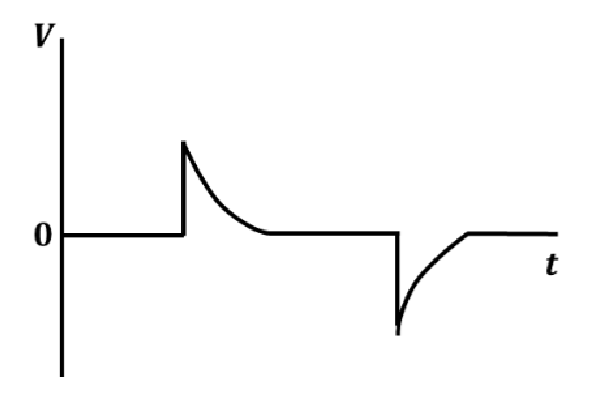
\includegraphics[width = \columnwidth]{2023/PH/37/figs/question.png}
    \caption{}
    \label{fig:ques_gate.ph.23.37}
\end{figure}

\begin{enumerate}[label = (\alph*)]
    \item
    \begin{minipage}[t]{\columnwidth}
        \begin{circuitikz}
    \draw(0, 0) to[short,*-*] ++ (4,0);
\draw (0,2) to[C,l=$0.1\mu F$, *-*] ++ (3,0) coordinate(a);
\draw (a) to[short,-*] ++ (1,0);
\draw (a) to[R, l_=$0.5k\Omega$,*-] ++(0,-2);

% Voltage labels
\draw (0,2) to[open,l_=V$_{in}$] ++(0,-2);
\draw (4,2) to[open,l=V$_{out}$] ++(0,-2);
\end{circuitikz}


    \end{minipage}
    \item
    \begin{minipage}[t]{\columnwidth}
        \begin{circuitikz}
    \draw(0, 0) to[short,*-*] ++ (4,0);
\draw (0,2) to[C,l=$1\mu F$, *-*] ++ (3,0) coordinate(a);
\draw (a) to[short,-*] ++ (1,0);
\draw (a) to[R, l_=$5k\Omega$,*-] ++(0,-2);

% Voltage labels
\draw (0,2) to[open,l_=V$_{in}$] ++(0,-2);
\draw (4,2) to[open,l=V$_{out}$] ++(0,-2);
\end{circuitikz}


    \end{minipage}
    \item
    \begin{minipage}[t]{\columnwidth}
        \begin{circuitikz}
    \draw(0, 0) to[short,*-*] ++ (4,0);
\draw (0,2) to[R, l = $0.5k\Omega$, *-] ++ (3,0) coordinate(a);
\draw (a) to[short,-*] ++ (1,0);
\draw (a) to[C,l_=$0.1\mu F$,*-*] ++(0,-2);

% Voltage labels
\draw (0,2) to[open,l_=V$_{in}$] ++(0,-2);
\draw (4,2) to[open,l=V$_{out}$] ++(0,-2);
\end{circuitikz}


    \end{minipage}
    \item
    \begin{minipage}[t]{\columnwidth}
        \begin{circuitikz}
    \draw(0, 0) to[short,*-*] ++ (4,0);
\draw (0,2) to[R, l = $5k\Omega$, *-] ++ (3,0) coordinate(a);
\draw (a) to[short,-*] ++ (1,0);
\draw (a) to[C,l_=$1\mu F$,*-*] ++(0,-2);

% Voltage labels
\draw (0,2) to[open,l_=V$_{in}$] ++(0,-2);
\draw (4,2) to[open,l=V$_{out}$] ++(0,-2);
\end{circuitikz}


    \end{minipage}
\end{enumerate}

\solution
\fi
\begin{table}[!h]
    \centering
    \begin{tabular}{|c|c|c|}
    \hline
       \textbf{Symbol}  & \textbf{Value} &  \textbf{Description}\\
    \hline
       $V_{in}(t)$  &  &  Input Voltage\\
    \hline
        $\mathcal{V}_{in}(f)$ & & Fourier Transform of $V_{in}(t)$\\
    \hline
        $V_{out}(t)$ & & Output Voltage\\
    \hline
        $\mathcal{V}_{out}(f)$ & & Fourier Transform of $V_{out}(t)$\\
    \hline
        $f$ & $1000Hz$ & Input Wave Frequency\\
    \hline
        $T$ & $\dfrac{1}{f} = 10^{-3} s$ & Input Wave Time Period\\
    \hline
        \multirow{2}{*}{$R$} & (a) $0.5k\Omega$ & \multirow{2}{*}{Resistance}\\
        \cline{2-2}
        & (b) $5k\Omega$ &\\
        \cline{2-2}
    \hline
        \multirow{2}{*}{$C$} & (a) $0.1\mu F$ & \multirow{2}{*}{Capacitance}\\
        \cline{2-2}
        & (b) $1\mu F$ &\\
        \cline{2-2}
    \hline
        $\tau$ & $RC$ & Time Constant\\
    \hline
        $Z$ & $R + \frac{1}{sC}$ & Impedance\\
    \hline
        $H(f)$ & $\frac{V_{out}}{V_{in}}$ & General Transfer Function\\
    \hline
        $H_{R}(f)$ & $\frac{V_{R, out}}{V_{in}}$ & Transfer Function for Resistor\\
    \hline
        $H_{C}(f)$ & $\frac{V_{C, out}}{V_{in}}$ & Transfer Function for Capacitor\\
    \hline
    \end{tabular}
    \caption{Given Parameters}
    \label{tab:1_gate.23.ph.37}
\end{table}


Input waveform is a square wave (\figref{fig:square_gate.ph.23.37}), so we take its Fourier Transform as shown in \figref{fig:square_fft_gate.ph.23.37}
\begin{align}
    V_{in}(t) &= 2\brak{2\sbrak{\frac{\brak{t-\frac{T}{4}}}{T}} - \sbrak{\frac{2\brak{t - \frac{T}{4}}}{T}}} + 1\\
    V_{in}(t) &\system{F} \mathcal{V}_{in}(f)
\end{align}
\begin{figure}[!h]
    \centering
    \begin{circuitikz}
    \draw(0, 0) to[short,*-] ++ (3,0);
    \draw (0,2) to[C,l=$\frac{1}{sC}$, *-] ++ (3,0) coordinate(a);
    %\draw (a) to[short,-*] ++ (1,0);
    \draw (a) to[R, l_=$R$,*-] ++(0,-2);
    
    % Voltage labels
    \draw (0,2) to[open,l_=V$_{in}$] ++(0,-2);
    \end{circuitikz}
    \caption{Series RC Circuit in s-domain}
    \label{fig:s-domain_gate.ph.23.37}
\end{figure}

\begin{align}
    s &= j2\pi f\\
    \implies Z &= R + \frac{1}{sC}\\
    &= R + \frac{1}{j2\pi f C}\\
    H(f) &= \frac{V_{out}}{V_{in}}
\end{align}

\begin{figure}[!h]
    \centering
    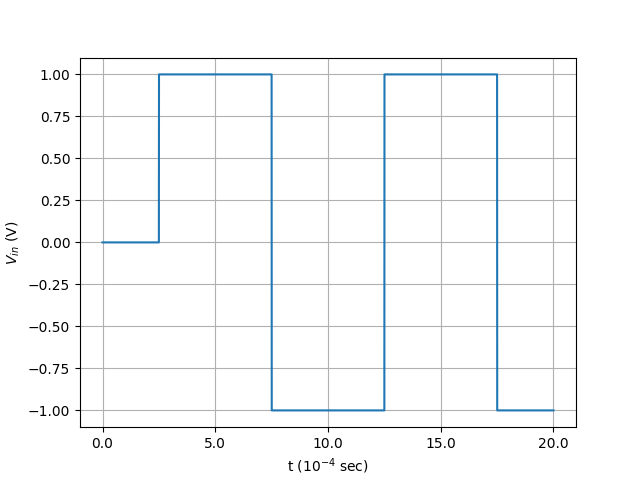
\includegraphics[width = \columnwidth]{2023/PH/37/figs/square.png}
    \caption{Input Square Waveform ($V_{in}(t)$)}
    \label{fig:square_gate.ph.23.37}
\end{figure}
\begin{figure}[!h]
    \centering
    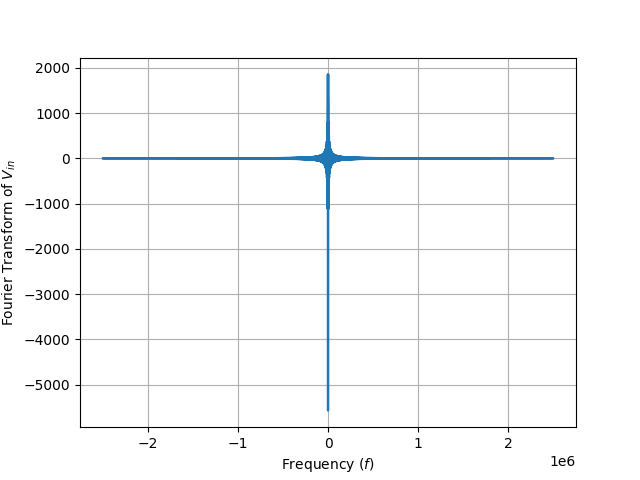
\includegraphics[width = \columnwidth]{2023/PH/37/figs/square_fourier.png}
    \caption{$\mathcal{V}_{in}(f)$ (Fourier Transform of $V_{in}(t)$)}
    \label{fig:square_fft_gate.ph.23.37}
\end{figure}
Across R,
\begin{align}
    H_{R}(f) &= \frac{R}{R + \frac{1}{j2\pi f C}}\\
    \implies \mathcal{V}_{out}(f) &= H_{R}(f)\mathcal{V}_{in}(f)
\end{align}

Across C,
\begin{align}
    H_{C}(f) &= \frac{\frac{1}{j2\pi f C}}{R + \frac{1}{j2\pi f C}}\\
    \implies \mathcal{V}_{out}(f) &= H_{C}(f)\mathcal{V}_{in}(f)\\
    \mathcal{V}_{out}(f) &\system{F} V_{out}(t)
\end{align}

$\mathcal{V}_{in}(f)$ was input into all four circuits and Inverse Fourier Transform was taken of the response. All responss are plotted below:
\begin{figure}[!h]
    \centering
    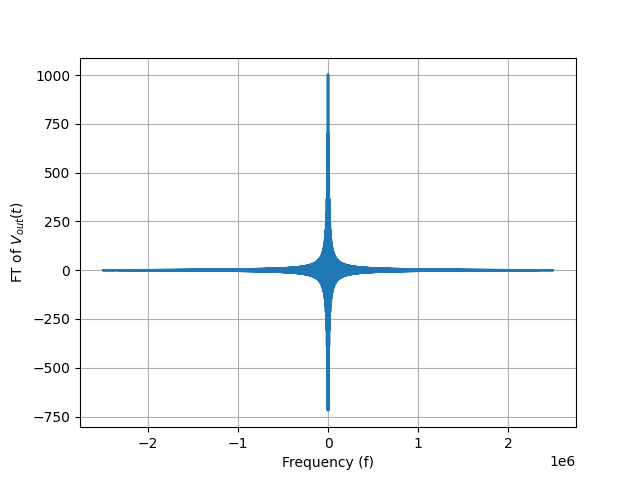
\includegraphics[width = \columnwidth]{2023/PH/37/figs/opt_a_ft.png}
    \caption{Opt A: Fourier Transform of $V_{out}(t)$}
    \label{fig:a_ft_gate.ph.23.37}
\end{figure}
\begin{figure}[!h]
    \centering
    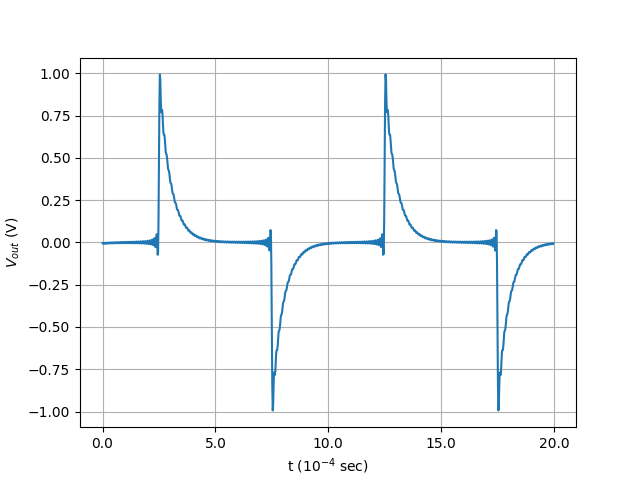
\includegraphics[width = \columnwidth]{2023/PH/37/figs/opt_a_res.png}
    \caption{Opt A: Response}
    \label{fig:a_res_gate.ph.23.37}
\end{figure}
\begin{figure}[!h]
    \centering
    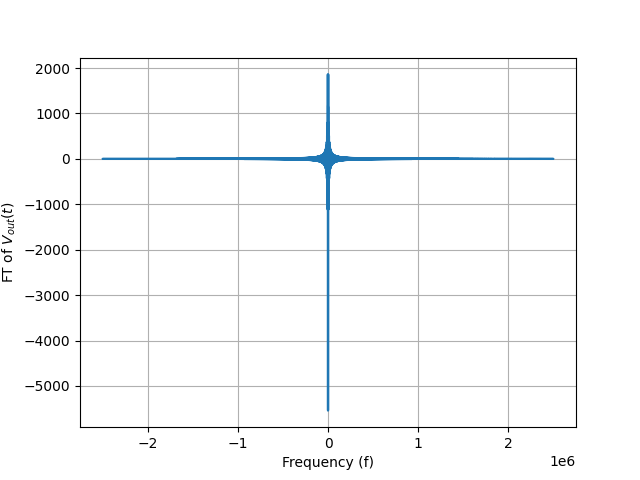
\includegraphics[width = \columnwidth]{2023/PH/37/figs/opt_b_ft.png}
    \caption{Opt B: Fourier Transform of $V_{out}(t)$}
    \label{fig:b_ft_gate.ph.23.37}
\end{figure}
\begin{figure}[!h]
    \centering
    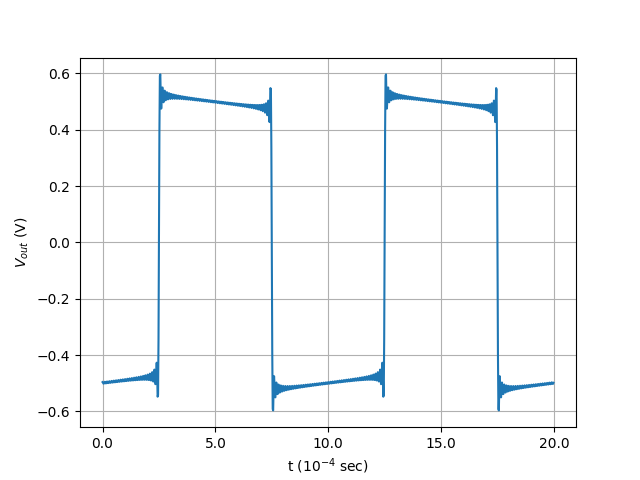
\includegraphics[width = \columnwidth]{2023/PH/37/figs/opt_b_res.png}
    \caption{Opt B: Response}
    \label{fig:b_res_gate.ph.23.37}
\end{figure}
\begin{figure}[!h]
    \centering
    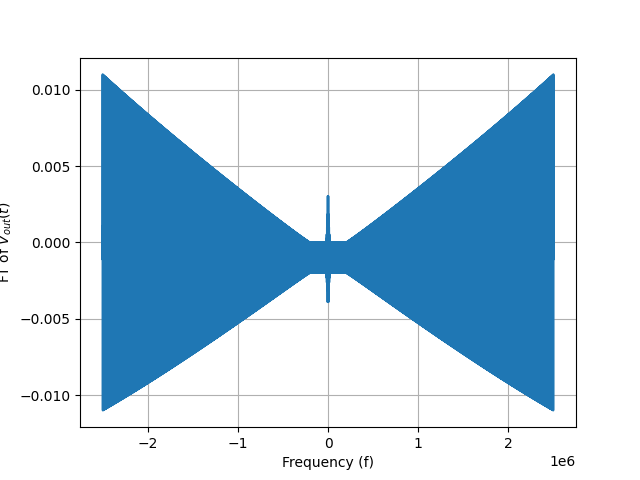
\includegraphics[width = \columnwidth]{2023/PH/37/figs/opt_c_ft.png}
    \caption{Opt C: Fourier Transform of $V_{out}(t)$}
    \label{fig:c_ft_gate.ph.23.37}
\end{figure}
\begin{figure}[!h]
    \centering
    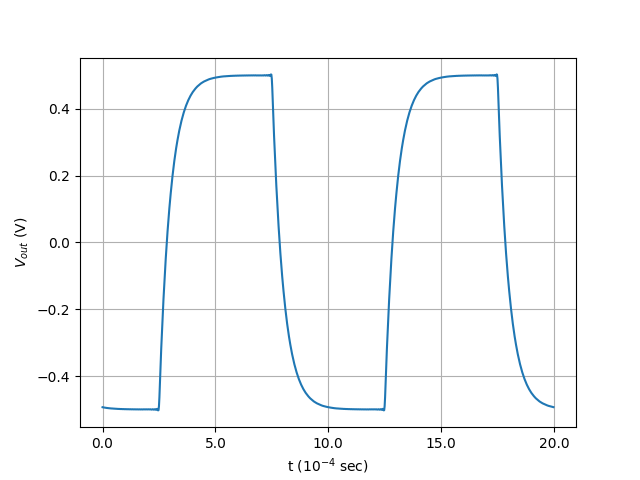
\includegraphics[width = \columnwidth]{2023/PH/37/figs/opt_c_res.png}
    \caption{Opt C: Response}
    \label{fig:c_res_gate.ph.23.37}
\end{figure}
\begin{figure}[!h]
    \centering
    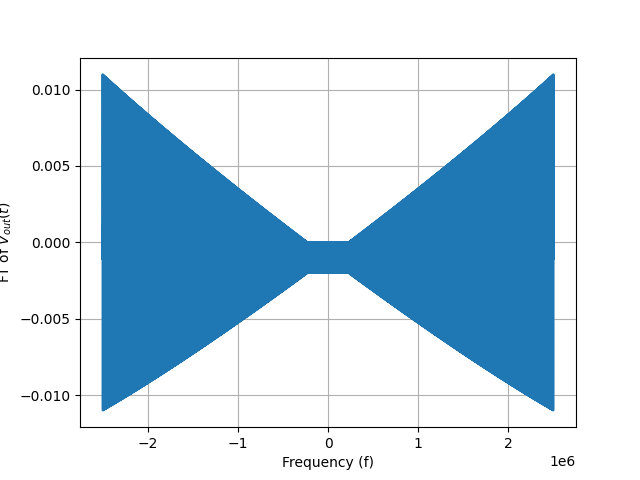
\includegraphics[width = \columnwidth]{2023/PH/37/figs/opt_d_ft.png}
    \caption{Opt D: Fourier Transform of $V_{out}(t)$}
    \label{fig:d_ft_gate.ph.23.37}
\end{figure}
\begin{figure}[!h]
    \centering
    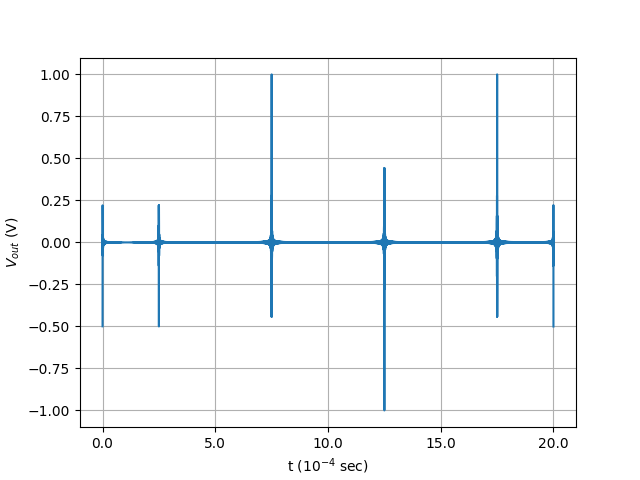
\includegraphics[width = \columnwidth]{2023/PH/37/figs/opt_d_res.png}
    \caption{Opt D: Response}
    \label{fig:d_res_gate.ph.23.37}
\end{figure}

As \figref{fig:a_res_gate.ph.23.37} resembles question \figref{fig:ques_gate.ph.23.37}, option (a) is the correct answer.
%\end{document}
